\documentclass[11pt]{article}
\usepackage{notes}
\usepackage{graphicx}
\def \scribe {Your Name}
\def \lecturer {Lecturer Name}
\def \lecturedate {\today}
\def \lecturenumber {1}
\def \lecturetitle {Lagrange Multipliers}
\def \coursename {Analytical Mechanics}
\def \coursenumber {PHYS 123}

\begin{document}
%\tableofcontents
\titleblock


\section{Block on a half-sphere}
Let's consider a basic kinematics asdf problem which we've solve previously using classical Newtonian methods.

\begin{example}{Block on a half-sphere}
Consider a half-sphere with a block sitting on its top. Using Lagrange multiplier methods, we can determine when the block will leave the surface of the half-sphere and at what angle from the vertical.

\begin{center}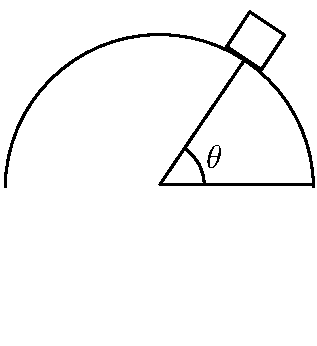
\includegraphics[width=0.25\textwidth]{fig1.pdf}\end{center}

\noindent First, consider the general lagrangian
\[ \lag = T-U \]
where
\[ \lag = \frac{1}{2} m \left(\dot{x}^2 + \dot{y}^2 + \dot{z}^2 \right) - mgz \]
so,
\begin{align*}
  \pd{\lag}{y} - \od{}{t} \left(\pd{\lag}{\dot{y}} \right) &= 0\\
  0 - \od{}{t} \left(m\dot{y} \right) &= 0\\
  m\ddot{y} &= 0
\end{align*}
Now, note that $y_0=0$ and $\dot{y}(0)=0$, so we can eliminate $y(t)$
\[ \lag = \frac{1}{2} m \left(\dot{x}^2 + \dot{y}^2 \right) - mgz \]
if we then switch to spherical coordinates
\[ \lag = \frac{1}{2} m \left( \dot{r}^2 + r^2 \dot{\theta}^2\right) - mgr \cos(\theta)\]
utilizing the constraint that $r-a=0$ such that
\[ \lag^* = \lag + \lambda(r-a) \]
where $\lambda$ is a force constraint only satisfied when the block is in contact with the surface of the half-sphere. If we use the Euler-Lagrange equation in terms of $\lag^*$
\begin{align}
  \pd{\lag}{r} - \od{}{t} \left(\pd{\lag^*}{\dot{r}} \right) &= 0 \nonumber\\
  mr\dot{\theta}^2 - mgr\cos(\theta) + \lambda - m\ddot{r} &= 0 \nonumber\\
  m\ddot{r} - mr\dot{\theta}^2 = \lambda - mg\cos(\theta) \label{eq:firstEqn}
\end{align}
where we can see that $\lambda$ in Eq. \eqref{eq:firstEqn} is in fact just the normal force. Now, we consider
\begin{align}
  \pd{\lag^*}{\theta} - \od{}{t} \left(\pd{\lag^*}{\dot{\theta}} \right) &= 0 \nonumber\\
  mgr\sin(\theta) - \od{}{t} \left(mr^2 \dot{\theta} \right) &= 0 \nonumber \\
  mgr\sin(\theta) - m\left(2 r \dot{r} \dot{\theta} + r^2 \ddot{\theta} \right) &= 0 \label{eq:secondEqn}
\end{align}
and, finally,
\begin{align}
  \pd{\lag^*}{\lambda} &= r-a = 0 \nonumber\\
  r &= a \nonumber\\
  \dot{r}(t) &= 0 \longrightarrow \ddot{r}(t) = 0 \label{eq:thirdEqn}
\end{align}
so, we can solve for the equation of motion with these three equations (i.e. Equation \eqref{eq:firstEqn}, \eqref{eq:secondEqn} and \eqref{eq:thirdEqn}) and applying the condition that $\dot{r}=0$ and $\ddot{r}=0$, we have
\begin{align*}
  -mr\dot{\theta}^2 &= \lambda - mg\cos(\theta)\\
  mgr\sin(\theta) - mr^2 \ddot{\theta} &= 0\\
  r &= a
\end{align*}
and then substituting in the condition $r=a$ and integrating over time
\[ \int_0^t mga \sin(\theta) \dot{\theta} \dif{t} = \int_0^t ma^2 \ddot{\theta} \dot{\theta} \dif{t} \]
and performing a change of base (i.e. $t \to \theta$)
\begin{align*}
  \int_0^\theta mga \sin(\theta)\, d\theta &= \int_0^\theta ma^2 \dot{\theta}\, d\dot{\theta}\\
  -mga\cos(\theta)\Big|_0^{\theta} &= \frac{1}{2} ma^2\dot{\theta}^2\\
  mga(1-\cos(\theta)) &= \frac{1}{2} ma^2 \dot{\theta}^2
\end{align*}
\end{example}

\section{Generalized Momentum}
Consider the Lagrangian
\begin{equation} \lag = \frac{1}{2} m \left(\dot{x}^2 + \dot{z}^2 \right) - mgz \end{equation}
and
\[ \pd{\lag}{\dot{x}} = m\dot{x} = \bv{p}_x \]
with the Euler-Lagrange equation
\begin{align*}
  \pd{\lag}{x} - \od{}{t} \left(\pd{\lag}{\dot{x}} \right) &= 0\\
  0 - \od{}{t} \left(\bv{p}_x \right) &= 0
\end{align*}
Considering translational invariance in the x-direction (i.e. conservation of momentum $\bv{p}_x$), we let
\[ \lag = \frac{1}{2}m \left(\dot{r}^2 + r^2 \dot{\theta}^2 \right) - mgr\cos(\theta) \]
In this case, $\bv{p}_r$ is not conserved since the momentum is dependent on the radius,
\begin{align*}
  \pd{\lag}{\dot{r}} &= m\dot{r} = \bv{p}_r\\
  \pd{\lag}{\dot{\theta}} &= mr^2 \dot{\theta} = \bv{p}_\theta
\end{align*}

\begin{figure}[ht!]
\centering
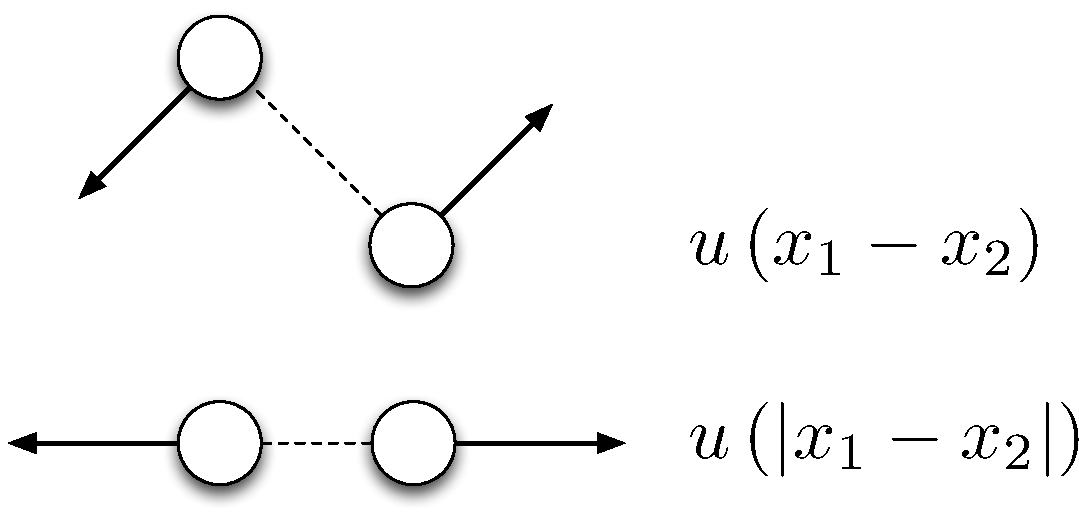
\includegraphics[width=0.3\textwidth]{fig2.pdf}
\caption{Our standard convention for momentum}
\label{fig:momentum}
\end{figure}
\end{document}
